\documentclass[fleqn,14pt]{article}

\usepackage[letterpaper,margin=0.75in]{geometry}

\usepackage{amsmath}
\usepackage{booktabs}
\usepackage{graphicx}
\usepackage{listings}
\usepackage{fancyhdr}
\usepackage{standalone}
\usepackage{pgfplots}
\usepackage{float}
\usepackage{csvsimple}
\usepackage{hyperref}
\usepackage{biblatex} %Imports biblatex package

% Bibliography
\addbibresource{all.bib}

% \include{data/reaction-time.csv}
 
\pgfplotsset{compat = newest}

\setlength{\parindent}{1.4em}

\pagestyle{fancy}


\begin{document}

\lstset{
  language=Python,
  basicstyle=\small,          % print whole listing small
  keywordstyle=\bfseries,
  identifierstyle=,           % nothing happens
  commentstyle=,              % white comments
  stringstyle=\ttfamily,      % typewriter type for strings
  showstringspaces=false,     % no special string spaces
  numbers=left,
  numberstyle=\tiny,
  numbersep=5pt,
  frame=tb,
}

\title{Lab Report}
\date{}
\def\theinstructor{Benjamin Koltai}



\author{Sidney Pauly}
\def\theuoastudentid{52104132}

\makeatletter

\let\thetitle\@title
\let\theauthor\@author
\let\thedate\@date


\makeatother




\fancyhf{}
\fancyhead[L]{Name: \theauthor}
\fancyhead[C]{ID: \theuoastudentid}
\fancyhead[R]{Instructor: \theinstructor}


% \maketitle

\begin{titlepage}
  \begin{center}
    \Large
    \textbf{\thetitle}
        
    \vspace{0.4cm}
    \large
    PX1015 - Experiment 5 - Counting and Timing
        
    \vspace{0.4cm}
    \textbf{\theauthor}\\
    \textbf{\theuoastudentid}

       
    \vspace{0.9cm}
    \textbf{Abstract}
  \end{center}
  The following experiments explore how digital counting can be used to collect very
  precise data from experiments.
  The experiments especially focus on how to use the digital counters to measure time intervals with a high
  degree of precision. This enabled measuring human reaction time,
  the frequency up to which a human can discriminate between flashes of a LED and the acceleration 
  of a falling ball. With this goal in mind, the experiment also lead
  to the exploration of the fundamentals that go into digital counting, like wiring
  up a circuit, using a function generator, using an oscilloscope and
  understanding how digital counters work.

  \vfill

  \begin{center}

    University of Aberdeen\\
    Scotland\\
    UK\\
    \thedate
    \vspace{0.4cm}
    \url{https://github.com/sidney-pauly/papers}
  \end{center}
\end{titlepage}


\section{Introduction}
Our modern world is heavily relying on electrical circuitry. More specifically integrated ones (ICs).
A common way such circuits operate is by utilizing a clock cycle. I. e. they update every pulse.
Today, the most advanced circuits (computers) run with frequencies (clock cycles per second) of up to
a few billion Hz (Ghz). A very basic circuit that can make use of such a clock cycles is a counter.
It simply add one for every
pulse it receives. If the pulses are at a constant frequency, this method can also be used to measure time.

\section{Theory}
\subsection{Electrical}

When wiring up any electrical circuitry some base theory is required. Ohms law,
tells us how resistance ($O$),
current ($I$) and voltage ($V$) are related:
$$
I = \frac{V}{R}
$$
The law is helpful, whenever one needs to figure out how to wire up a component that has limits
on either the current or voltage it can handle,
or how a resistor (i.e. any consumer) will affect the circuit. The current
is inversely proportional to the resistance. Thus, if we want to decrease the current we need
to increase the resistance.\\
Then, there is also the laws on how to combine resistors: \\
\\
Series:
$$
R_T = R_1 + R_2
$$
Parallel:
$$
\frac{1}{R_T} = \frac{1}{R_1} + \frac{1}{R_2}
$$
(equations for two resistors)\\
\\
Resistors combined in parallel yield decreased resistance values.
If they are combined in series their resistance will add up instead.

\subsection{Binary counting}
Digital circuits have two basic states: off and on (0 and 1). They cannot handle other values.
Counting in base-10 (0-9), like humans do, is not possible for digital circuits. Base-2/binary (0-1) is used 
instead. One digit of a binary number is called a bit.\\
Some examples for binary numbers with
their decimal counterparts are:

\vspace{0.5cm}
\begin{tabular}{lc}
  Binary & Decimal\\
  \midrule
  $0000\_0100$ & 4\\
  $0000\_1000$ & 8\\
  $0001\_1000$ & 24\\
\end{tabular}
\vspace{0.5cm}


Translating from binary to decimal is straightforward. It can be done using the following formula:
$$
d=n_0\ast2^0+n_1\ast2^1+\ldots+n_m\ast2^m
$$
Where n is the corresponding binary digit.

\subsection{Kinematics}

Furthermore, some kinematic equations will be used to calculate the acceleration
of a falling object (assumed to have constant acceleration). Using two sections, within which
the object's velocity is measured,
the acceleration can be calculated :\\
\\
Average velocity
$$
v_{avg}=\frac{l}{t}
$$

We can then take the difference between $v_1$ and $v_2$ to get $\Delta v$ as well as the difference between
$t_1$ and $t_2$ to get $\Delta t$.\\
\\
Therefore
$$
a = \frac{\Delta v}{\Delta t}
$$
Plugging everything in:
$$
a = \frac{2(\frac{l_2}{t_2}-\frac{l_1}{t_1})}{t_1+t_2}
$$

\section{Experimental Procedure}
\subsection{Wiring up an LED}
To test and verify the electrical setup, the first step was to wire up a LED. For quick reconfiguration of
the circuits a breadboard was used. Safely operating a LED requires:
\begin{enumerate}
  \item Direction: LEDs are diodes (LightEmittingDiode) so they only let electrons pass in one direction
  \item Current: LEDs can only be used up to a certain current, beyond which they get damaged.
\end{enumerate}
Finding out the direction was done by testing which way the LED lit up. This is safe as the LED is not damaged
if wired up the wrong way around. To limit the current flowing through the LED a resistor wired up in
series was used. As can be seen from $I = \frac{V}{R}$ the current can be decreased by increasing the
resistance. The documentation on the LED called for a $330\Omega$ resistor. As such a resistor was not
available, instead two $160\Omega$ were used in series instead. After connecting a 5 volt power supply
the LED lit up.

\subsection {Function generator and Oscilloscope}
The next step was trying out the function generator. As it had a 5 volt output as well, it could be used as
a direct substitute for the power supply. As the circuits used later needed square waves to work properly,
that setting was also chosen to test the LED. To verify that everything worked properly, a low frequency of 1Hz
was chosen, for easy detection. After turning on the function generator the LED started
to blink.\\
\\
Next, the oscilloscope was brought out to take a closer look at the output of the function generator. It
was wired up as illustrated in the manual:
\begin{figure}[h]
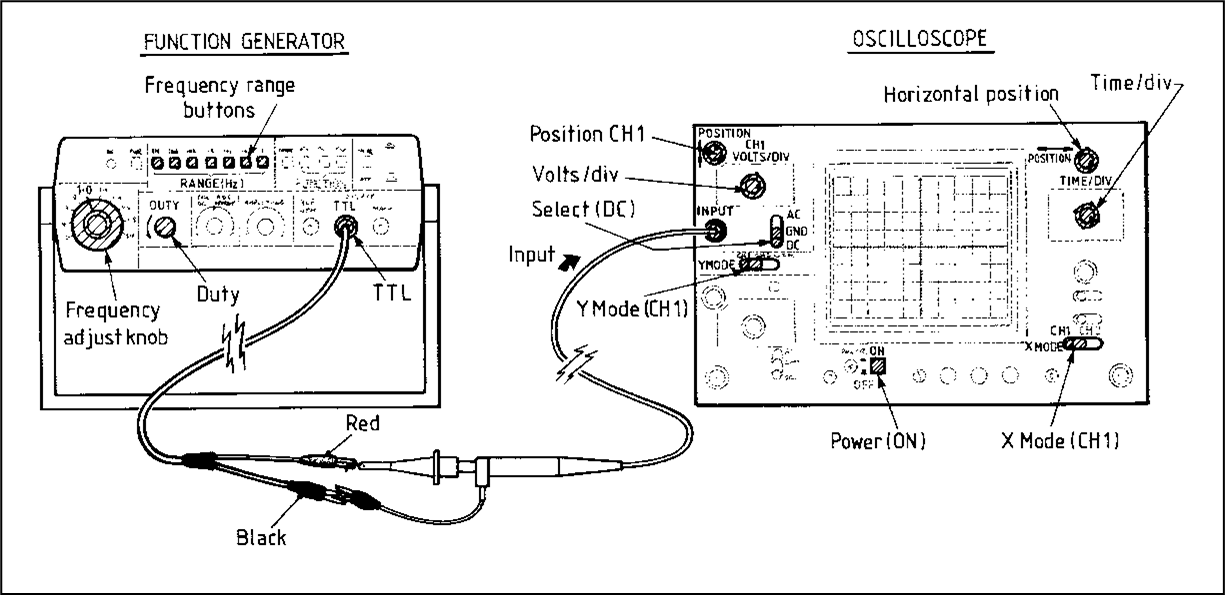
\includegraphics[width=16cm]{images/Oscilloscope.png}
\caption{Function Generator wired up to Oscilloscope \cite{ross}}
\label{fig:figure1}
\end{figure}

First the Time/div knob was set to a very high value, this resulted in just a spot showing on the
oscilloscope. By centering (Position CH1) that point (0V) the oscilloscope could be calibrated. After that the
Volts/div slider was set such that it lay within the 5V range of the function generator. This resulted
in two spots showing. In a third step the Time/div slider was set such that the time interval was close
to what the function generator was producing as an output. The result was a square wave showing on the
oscilloscope:

\begin{figure}[H]
  \centering
  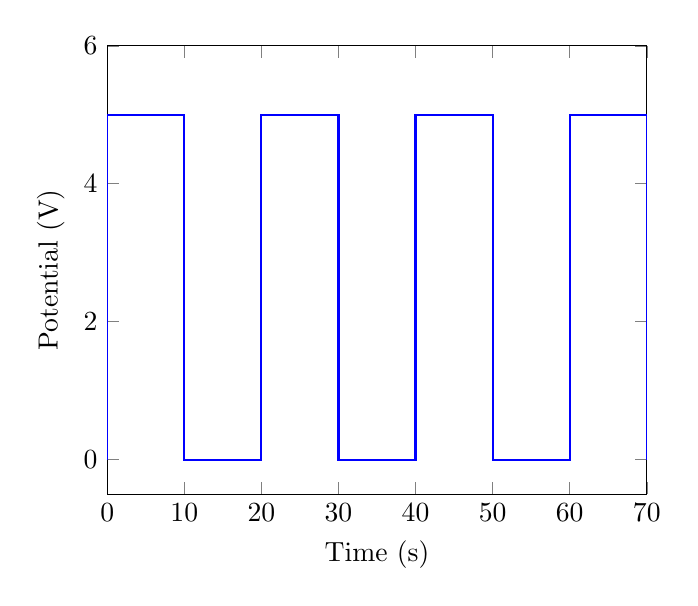
\begin{tikzpicture}
 
    \begin{axis}[
        ylabel={Potential (V)},
        xlabel={Time (s)},
        xmin = 0, xmax = 70,
        ymin = -0.5, ymax = 6]
        \addplot+[thick,mark=none,const plot]
        coordinates
        {(0,0) (0,5) (10,0) (20,5) (30,0) (40,5) (50,0) (60,5) (70,0)};
    \end{axis}
     
  \end{tikzpicture}
  \caption{Idealized plotted square wave}
  \label{fig:figure2}
\end{figure}

Increasing the frequency of the function also changed how long each of the pulses on the oscilloscope 
were showing on the screen.
The setup allowed to test the maximum frequency perceivable by a human. The
frequency was set to 100Hz (No perceivable flickering), and slowly lowered until flickering could be perceived.

\subsection{Counting}
Dfferent counting circuits were wired up instead of the LED.
All of the different counter circuits had two pins to connect
a clock. The function generator was connected to those pins as such a timing device. The first circuit had
only two buttons: start and reset. There were no additional pins. A bar of LEDs displayed the current
count. \\
\\
Afterwards a counting device with a
7-segment display was wired up. It offered an additional switch to either use the direct output
of the counting IC or put it through a binary to BCD translation IC. BCD stands for  Binary-Coded-Decimal.
BCD uses 4 bits per decimal digit to represent it. 4 bits are used as $2^4=16 > 9$. \\
\\
A circuit that counted the number of pulses within a given time period (switchable between
0.1s, 1s or 10s) connected to the previous setup. By connecting the function generator,
the number of pulses per second were evaluated.\\
\\
Lastly, a counting device with four 7-segment displays was connected. It counted up to 9999 ($10^4-1$). In
addition, it also had a start, stop and a reset button with electrical pins. Grounding them triggered
the corresponding action. The stop button was wired to a hand-held thumb-actuated button. The function
generator was then set to a 1000Hz such that a value of 1 on the counter would represent 1 milliseconds.
The start switch was covered up, the counter reset and the experimenter prepared to press the start button.
The test subject held the stop button; tasked to press it as soon as they could see the counter
starting to count.
This way, the reaction time of the test subject could be assessed.

\subsection{Measuring Gravity}


\begin{figure}[H]
  \begin{center}
    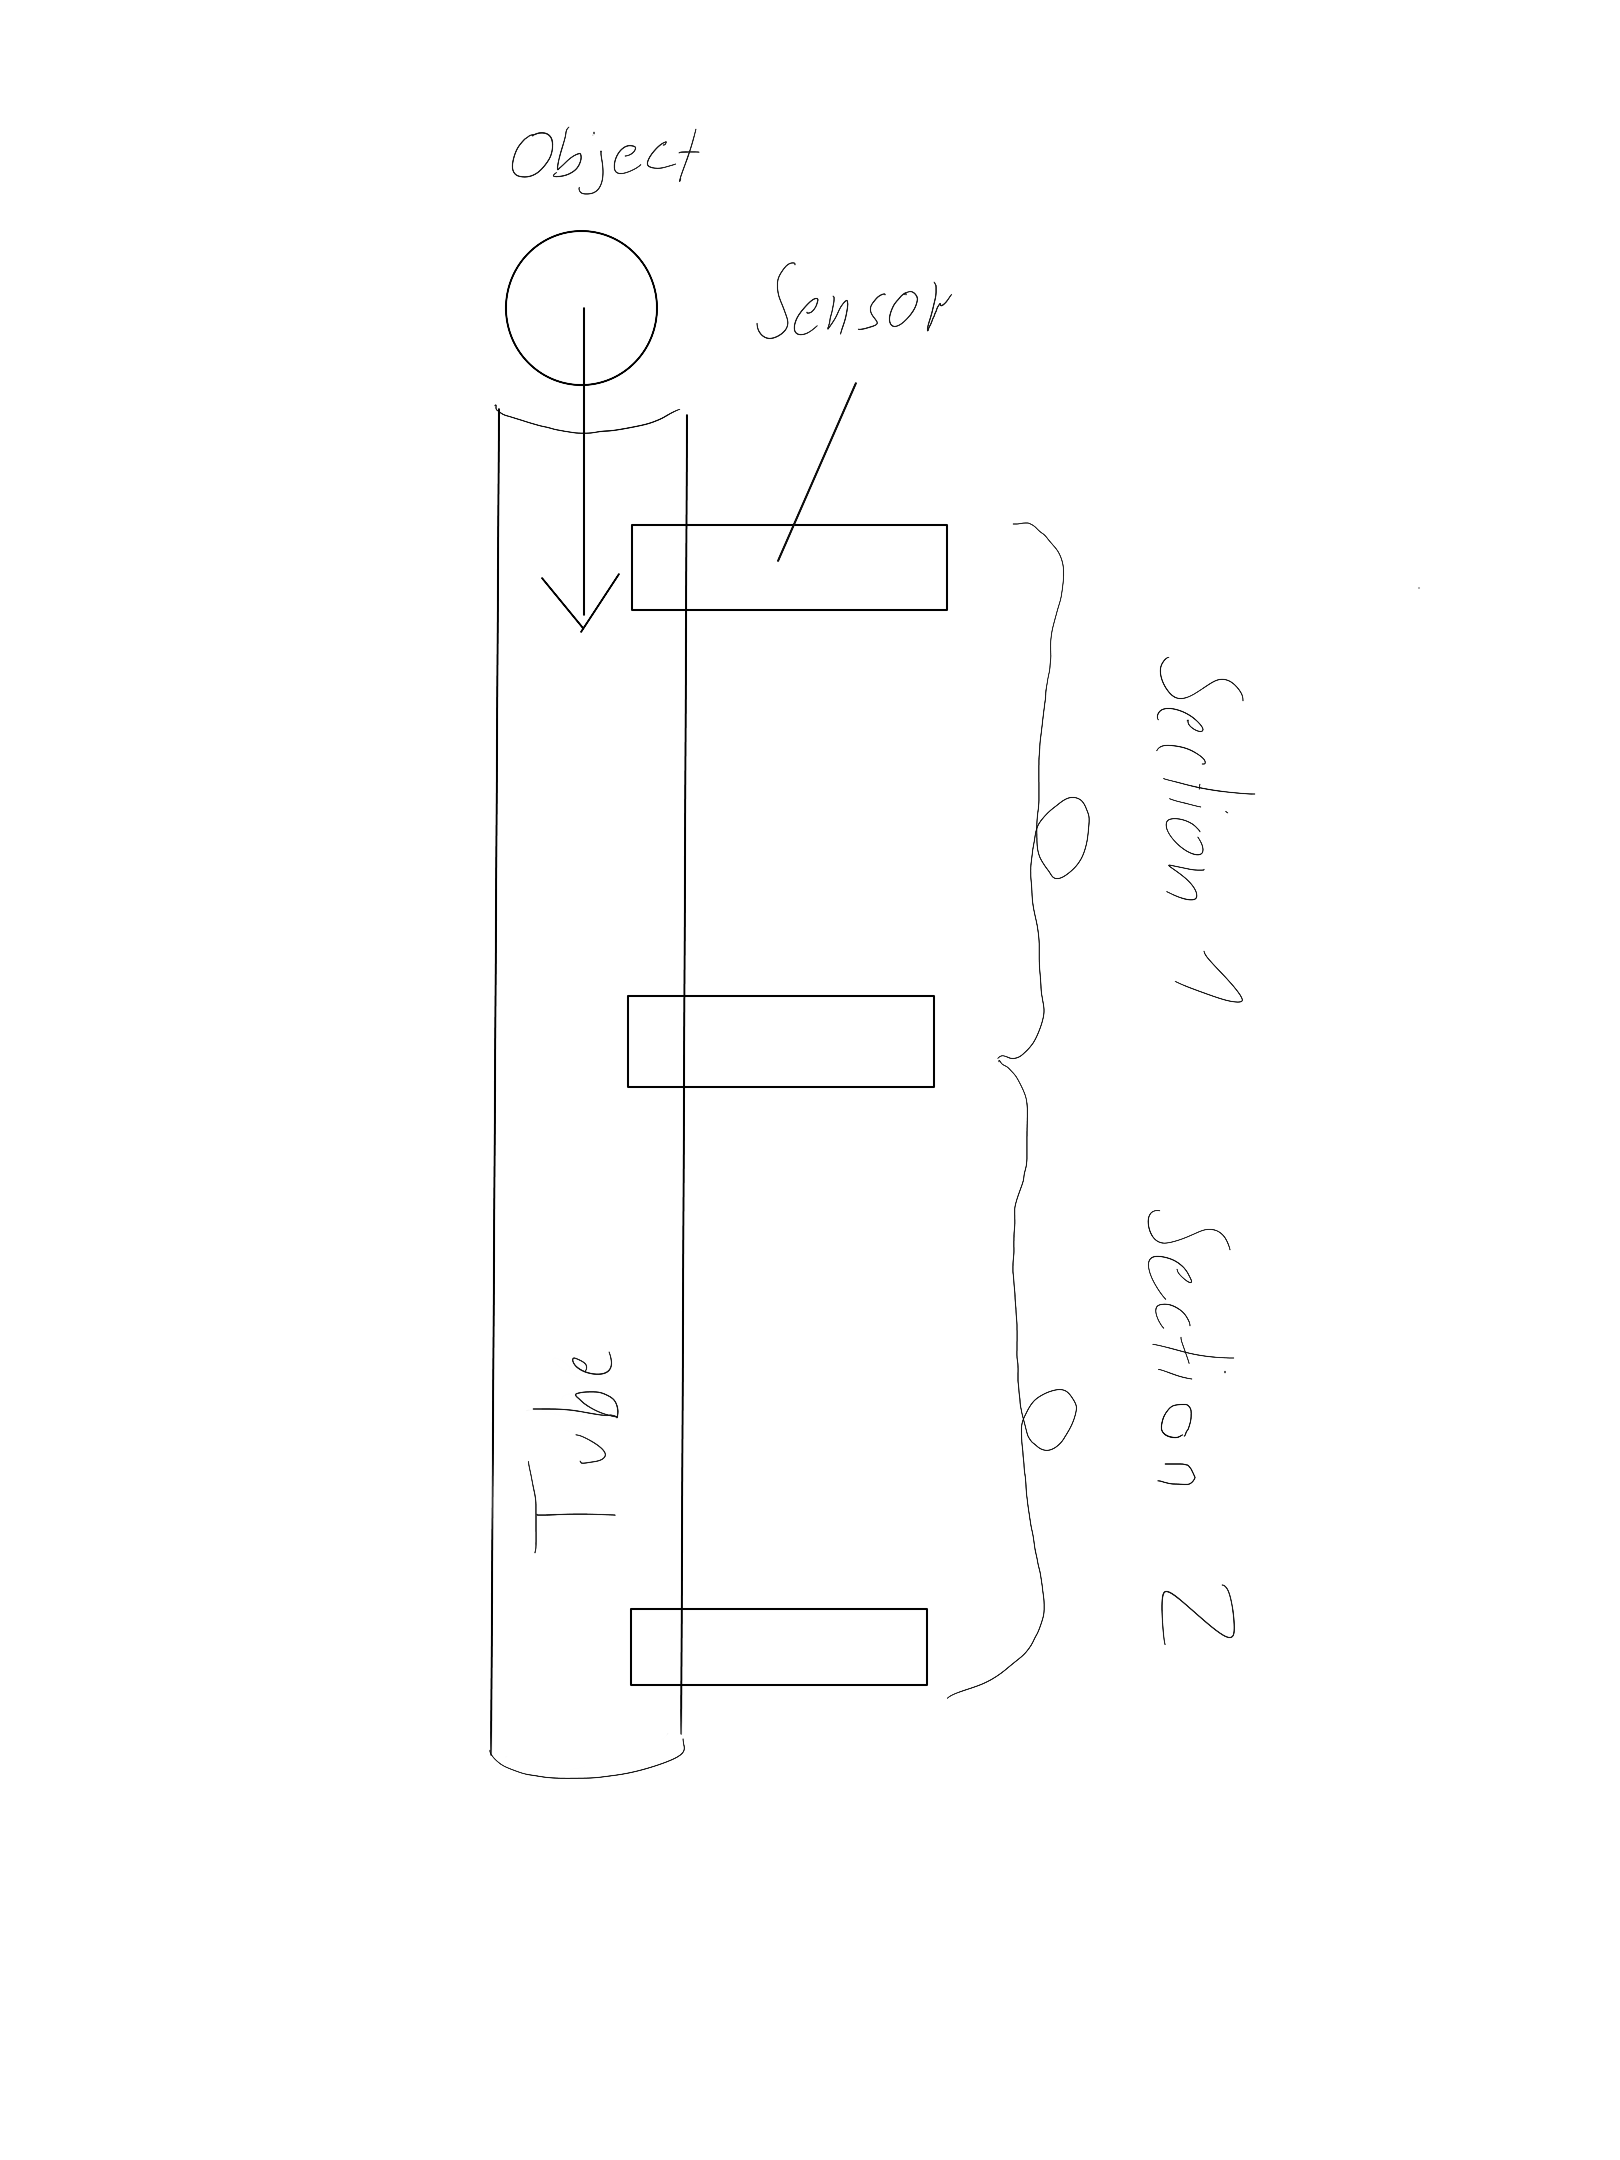
\includegraphics[width=10cm]{images/drop-tower.png}
    \caption{Experimental setup}
    \label{fig:figure_drop_tower}
  \end{center}
\end{figure}

With all circuits setup and verified working, the gravitational
acceleration of different objects was measured. To do so, a drop tower with three gates was used, with
four previously introduced 7-segment counters were used. The gates of the tower were then wired up such
that gate one was connected to the start pin of the counter one, gate 2 to the stop pin of counter one as
well as the start pin of counter two and gate three to the stop pin of counter two. Thus creating a
setup that could count the number of pulses passing while an object traveled between the respective gates.
By setting the function generator to produce an output of 1000Hz this could then be translated into time.
With this setup different objects were dropped down the tube. Balls of two sizes and four different materials
were used. A small pen as an object having minimal air resistance was also tested. 
To obtain additional precision the frequency displayed on the function generator was recorded to be applied as
a corrective term. To improve accuracy further a run with done with the function generator set to 10,000Hz.



\section{Experimental Results}

\subsection{Human perceivable frequencies}

\vspace{0.5cm}
\begin{tabular}{lc}
  Person & Frequency (Hz)\\
  \midrule
  Sidney & 36\\
  Bray & 30\\
\end{tabular}
\vspace{0.5cm}

\subsection{Digital Counting}
\paragraph{BIN/BCD circuit}
While testing the BIN/BCD switchable counting circuit, it was observed that the 7-segment display did not
go through the numbers correctly all of the time. If the switch was set to BCD the counting worked correctly
with the display going form 0 to 9 and then resetting. Setting the switch to BIN this did not work properly.
The display was instead counting up to 6 and then did show different numbers in a random seeming way.

\paragraph{Function Generator output verification}
When connecting the function generator to the 1s resetting counter, different frequencies on
the function generator were configured. The observation were as follows:

\begin{enumerate}
  \item When changing the frequency on the function generator, it took a while for the actual frequency to stabilize.
  \item When pressing any of the buttons or moving the cables of the counting circuit the same phenomenon
  was observed
  \item Once settled the counter showed the same value as the reading on the oscilloscope up to 1 count
  of difference
\end{enumerate}

\subsection{Reaction Time}

\vspace{0.5cm}
\begin{tabular}{l|ccccc|cc}
  Person & 1 & 2 & 3 & 4 & 5 & Average & Standard Deviation\\
  \midrule
  Sidney & 242.3 & 225.5 & 156.5 & 163 & 228.7 & 203.2 & 40.2\\
  Bray & 189.5 & 330.5 & 252.9 & 150.2 & 171.1 & 218.84 & 73.3\\
\end{tabular}
\vspace{0.5cm}

\subsection{Gravity}

\begin{tabular}{lcccccc}
  Material & $t_0$ & $t_1$ & Correction & $t_{0_{corrected}}$ & $t_{1_{corrected}}$ & g\\
  \midrule
  Rubber & 0.175 & 0.1 & 0.996015936 & 0.174302789 & 0.099601594 & 9.425604156\\
  Wood & 0.179 & 0.1 & 0.996015936 & 0.178286853 & 0.099601594 & 9.567281072\\
  Plastic & 0.182 & 0.104 & 0.996015936 & 0.1812749 & 0.103585657 & 8.714500884\\
  Wood small & 0.18 & 0.1 & 0.996015936 & 0.179282869 & 0.099601594 & 9.600152381\\
  Glass small & 0.181 & 0.099 & 0.996015936 & 0.180278884 & 0.098605578 & 9.884637057\\
  Metal & 0.181 & 0.099 & 0.996015936 & 0.180278884 & 0.098605578 & 9.884637057\\
  Glass  & 0.18 & 0.099 & 0.996015936 & 0.179282869 & 0.098605578 & 9.853528837\\
  Dart & 0.1441 & 0.097 & 1.005025126 & 0.144824121 & 0.097487437 & 8.302050935\\
  Metal (10kHz)& 0.1765 & 0.0981 & 1.005025126 & 0.177386935 & 0.098592965 & 9.794882365\\

\end{tabular}
\vspace{0.5cm}


\section{Discussion and Analysis}

\subsection{Human perceivable frequencies}
No hard boundary could be observed between the LED flickering and being on continuously. In the transition
the LED was neither perceived to flicker nor being on continuously.
The perceived effect, might, in appearance, be comparable to candle light. There is flickering, tough not
in the 20Hz-40Hz configured, instead perceived as 5-10Hz. Possible explanations include, but are not limited
to:

\begin{enumerate}
  \item There is an error in the electronics and the LED sometimes stays off for longer than commanded.
  \item Past a certain frequency, the flashes are too fast for a person to perceive them. Instead, only
  e.g every other flash is caught. This is comparable to the shutter in a camera that, depending on the set frequency
  either catches the light being on or off. Of course, human eyes have no shutter, but this could be something
  happening in the brain.
\end{enumerate}

Hypothesis one is less likely due to the supposed slip-ups not being observable
at other frequencies. Also the other measurements conducted with the oscilloscope did not reveal anything
of the sort.

\subsection{Digital Counting}
While testing the 7-segment display counter wired behavior was observed while the switch was set to BIN.
A possible explanation is that the 7-segment display driver IC expects a BCD input and thus if that translation
does not happen, still assumes the input is BCD. This can be confirmed by looking at what the 7-segment display
would output in such a case:

\vspace{0.5cm}
\begin{tabular}{lccc}
  Binary & BCD & Actual Decimal & Displayed Decimal\\
  \midrule
  $0000\_0001$ & 0001 & 1 & 1\\
  $0000\_0010$ & 0010 & 2 & 2\\
  $0000\_0011$ & 0011 & 3 & 3\\
  $0000\_0100$ & 0100 & 4 & 4\\
  $0000\_0101$ & 0101 & 5 & 5\\
  $0000\_0110$ & 0110 & 6 & 6\\
  $0000\_0111$ & 0111 & 7 & 7\\
  $0000\_1000$ & 1000 & 8 & 8\\
  $0000\_1001$ & 1001 & 9 & 9\\
  $0000\_1010$ & 0001 0000 & 10 & 2\\
  $0000\_1011$ & 0010 0000 & 11 & 3\\
  $0000\_1100$ & 0011 0000 & 12 & 4\\
\end{tabular}
\vspace{0.5cm}

It can be seen that as soon as the counter reaches double digits, it would be different from the actual
number. While it cannot be confirmed that this is the exact behavior exhibited by the counter (as the
sequence produced by it was not recorded), it is likely that this or something similar happened.\\

\subsection{Reaction Time}
With the limit of only having two human test subjects the results of the experiment are quite limited.
Also it has to be noted that the recorded numbers might differ slightly, because of the jitter of the function
generator that could be observed if any of the buttons were being pressed. This can be neglected
as the jitter seemed to be happening equally in both directions and should therefore average out
over the runs. Additionally, the standard deviation is in any case a lot higher than what the jitter alone
could explain. This is because the jitter was observed to be in the single millisecond domain, while the
standard deviation is in the 100 millisecond domain.\\
\\
First the reaction time of 20
year old test subjects appears to be in the 200-220 millisecond range. This is close to the value stated in
online resources \cite{wiki} . The high value of the standard deviation indicates that human reaction time is
inconsistent. The most likely explanation being the variable human attention span.

\subsection{Gravity}
The last experiment was likely most affected by the jitter, pointed to by:
$$
\Delta a \propto \frac{1}{\Delta t^2}
$$
Slight variations in the measured time have a significant impact on the measured acceleration. To minimize
this problem, a correction term was applied. It came from the difference between the set and observed frequencies.
This correction could only account for a general offset,
not for the jitter induced by the falling object triggering the gates.\\
Other factors hindering the precision of the experiment are the imprecise measurement of the tube length (only
accurate to $10^{-1}m$) as well as the tube itself potentially trapping air and thus causing a air cushion to
be formed. \\
\\
Also potentially affecting the results is the time resolution of the counter. With the function generator
set to 1 kHz only time-steps of 1 millisecond can be recorded. To increase precision, the function generator's
frequency was increased to 10 kHz for the last trial, giving a 10 times improved time resolution.
The aforementioned jitter, might jeopardize the improved resolution as the jitter's magnitude being ten times
greater. 
\\
If this experiment was to be repeated, most effective would be to reduce the jitter. This might be achieved by 
modifying the circuits (e.g. adding a capacitor), so that any electrical effects induced by the switching
are reduced. Additionally, doing multiple trials with the same setup might improve the situation as well.\\
\\
As expected from theory, heavier materials as well as bigger solid spheres fall faster.
This can be derived as follows:\\
\\
Air resistance:
$$
F_a \propto A
$$
Force due to gravity:
$$
F_g = g m
$$
as the mass of a sphere is given by
$$
m = \rho \frac{4}{3} \pi r^3
$$
thus,
$$
F_g = g \rho \frac{4}{3} \pi r^3
$$
while the area is described by
$$
A =  4 \pi r^2
$$
thus,
$$
F_a \propto r^2
$$
while
$$
F_g \propto r^3
$$
therefore $F_a >> F_g$ for big $r$
and
$$
F_g \propto \rho
$$
(With $F_a$ as air resistance, $F_g$ as force due to gravity and
$F_{total} = F_g - F_a$)\\
\\
In some
of the trials, the measured acceleration was higher than what is commonly quoted as $g$ ($9.1ms^-2$).
This might point to a systematical error within the experiment that leads to a shift of the measured values, above
the actual present acceleration. Curiously, the last trial where the function generator was set to 10 kHz was
a lot closer to the expected value of $g$ (note that a big metal ball was used, thus reducing the effect of 
air resistance as shown). Without making more measurements, it is not conclusive if this was just a statistical
fluke or actually the result of the improved time resolution.

\section{Conclusion}
Overall, it could be observed that using electronic circuits and counting devices allows for a wider range
of experiments to be conducted. This is especially true for processes that happen fast and can thus not
be fully grasped by mere unaided observation. It is also clear that electronic counting/measuring allows
for a lot higher time-resolution. This is highlighted by the fact that the
highest achievable time-resolution within the experiment was 0.1ms (10kHz), while the highest time-resolution
that was achieved by a human was around 33ms (30Hz).

\printbibliography

\end{document}